\documentclass[a4paper,12pt]{article}


\usepackage{setspace}
\usepackage{xcolor}
\usepackage{graphicx}
\usepackage{geometry}
\usepackage{float}
\usepackage{titlesec}
\usepackage{subfigure}
\usepackage{caption}
\captionsetup{figurewithin=section}
\usepackage{amsmath}
\usepackage{enumitem}
\usepackage{amssymb}

\begin{document}

\title{\textbf{Homework 3}}
\author{Yunian Pan}
\maketitle{}

\section{Problem 1: Kernel}

\begin{enumerate} [label = $\bullet$]
   \item $k(u,v) = \alpha k_1(u,v) + \beta k_2(u,v), \   for \ \alpha, \beta \geq 0$
   
   Through building vector blocks:
      \begin{align}
      k(u,v) & =  \alpha\phi_1(u) \cdot \phi_1(v) + \beta \phi_2(u) \cdot \phi_2(v)  \nonumber \\ 
       & = (\sqrt{\alpha} \phi_1(u) , \sqrt{\beta} \phi_2(u) ) \cdot (\sqrt{\alpha} \phi_1(v) , \sqrt{\beta} \phi_2(v) ) \nonumber \\
       & = \phi(u) \cdot \phi(v) \nonumber
      \end{align}
     Which holds symmetric and positive semi-definite property.
      
   \item $k(u,v) = k_1(u,v) k_2(u,v)$
     \begin{align}
      k(u,v) & =  \phi_1(u) \cdot \phi_1(v) \times \phi_2(u) \cdot \phi_2(v)  \nonumber \\ 
       & = ( \sum_{i}f_i(u)  f_j(v))  ( \sum_{j}g_j(u)  g_j(v)) \nonumber  \\
       & = \sum_{ij}f_i(u)g_j(u)  f_i(v) g_j(v) \nonumber \\
       & = \sum_{m} \Phi_m(u) \Phi_m(v)   \qquad (\Phi_m(x) = f_i(x)g_j(x), \ m = ij)\nonumber \\
       & = \phi(u)\cdot \phi(v ) \nonumber 
      \end{align}
      Which is symmetric for it keeps the same form when u and v get exchanged.
      
      Consider the positive semi-definiteness, since $k_1(u,v)$ and $k_2(u,v)$ are both positive semi-definite, the Gram matrix K whose entries are the product of $K_{1,ij}$ and $K_{2,ij}$ is also positive semi-definite. ($K_1$ and $K_2$ are  Gram matrix of $k_1$ and $k_2$ inner product for all $u,v\in \chi$.)
   
   \item $k(u,v) = k_1(f(u), f(v)) , \ where \ f: \chi \rightarrow \chi$
     \begin{align}
      k(u,v) & =  \phi_1(f(u)) \cdot \phi_1(f(v))  \qquad \qquad define \ \phi(x) = \phi_1(f(x)) \nonumber \\
      & = \phi(u) \cdot \phi(v) \nonumber
     \end{align}
     Which inherits symmetric and positive semi-definite property from $k_1$.
     
   \item $k(u,v) = g(u)g(v), \ where \ g: \chi \rightarrow \mathbb{R}$
   
   Obviously here $\phi(u) = g(u)$, $k(u,v)$ is a valid symmetric kernel for $k(u,v) = <\phi(u) ,\phi(v)>$.
   
   All we need to do is check the positive semi-definiteness of Gram matrix $K_{ij} = g(x_i) g(x_j)$ for $\{x_i, x_j \in \chi\}$, $K = G G^{\mathsf{T}}$. we can find $G$ and any other $n-1$ vectors which are in the orthogonal complement of $G$, with eigenvalues $\lVert G\rVert^2 \ and \ 0 (n - 1 \ multiplicity)$. So $K$ is positive semi-definite. 
   
   \item $k(u,v) = f(k_1(u,v)), \ where \ f \ is \ a\ polynomial\ with \ positive \ coefficients$
   \begin{align} 
   &k(u,v) = \sum_{i} c_i (\phi_1(u) \phi_1(v))^i \quad  c_i \geq 0 \nonumber \\
   &apply\ the\ second \ result\ repeatedly: \nonumber \\
   &k(u,v) = \sum_{i} c_i k_i(u,v) \quad  c_i \geq 0 \nonumber \\
   &apply \ the \ first\  result\ repeatedly:\nonumber \\
   &k(u,v) \ is\ a \ valid \ kernel . \nonumber 
   \end{align}
   
   \item $k(u,v) = \exp(k_1(u,v))$
    \begin{align}
      k(u,v) & =  \lim_{n \rightarrow \infty} \sum_{i = 0}^{n} \dfrac{k_1(u,v)^i}{i!}\nonumber \\
      & = f(k_1(u,v)) \ where \ f \ is \ a\ polynomial\ with \ positive \ coefficients \nonumber
     \end{align}
    Therefore $k(u,v)$ is a valid kernel.
    
   \item $k(u,v) = \exp(\frac{-\lVert u - v \rVert^2}{\sigma^2})$ 
     \begin{align}
      k(u,v) & =  \exp(- \frac{\lVert u\rVert^2}{\sigma^2})  \times \exp(\frac{2 \times u \cdot v}{\sigma^2}) \times \exp( -\frac{\lVert v \rVert^2}{\sigma^2})  \nonumber \\
      & = g(u)g(v) \exp(\phi(u) \cdot \phi(v))  \nonumber 
     \end{align}
     
    Where $g(x) = \exp(-\frac{\lVert x\rVert^2}{\sigma^2})$ and $\phi(x) = \frac{\sqrt{2} x}{\sigma}$, thus apply the conclusion that $k(u,v) = k_1(u,v) k_2(u,v)$, $k(u,v) = g(u)g(v), \ where \ g: \chi \rightarrow \mathbb{R}$ and $k(u,v) = \exp(k_1(u,v))$ are all valid kernels,  $k(u,v) = \exp(\frac{-\lVert u - v \rVert^2}{\sigma^2})$ is also a valid kernel.
\end{enumerate}

\section{Problem 2: SVMs}

For linear kernel, we only need to adjust the cost to see the performance of different SVMs, there's no error when cost ranges from 1 to 100 , so I extended the cost value $C$ to $10^{-6} \to 10^{6}$. As for polynomial kernel and rbf kernel, I used the same cost range with polynomial order $p$ ranging  from 1 to 13 and variance $\sigma$ ranging from $10^{-6}$ to $10^{6}$.

Using the signum function, the performances are shown as in $\ref{ls}$, $\ref{ps}$, $\ref{rs}$.
\begin{figure}
\centering
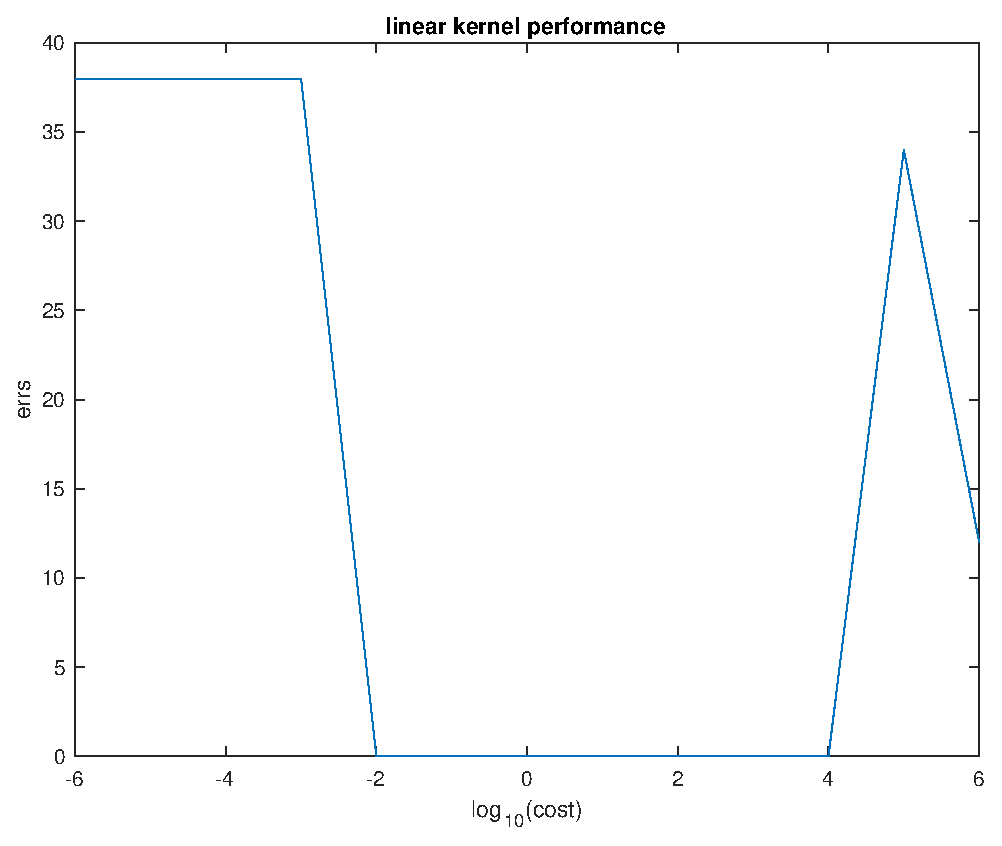
\includegraphics[width=.7\textwidth]{figure/linear_performance_s.eps}
\caption{linear performance signum}
\label{ls}
\end{figure}

\begin{figure}
\centering
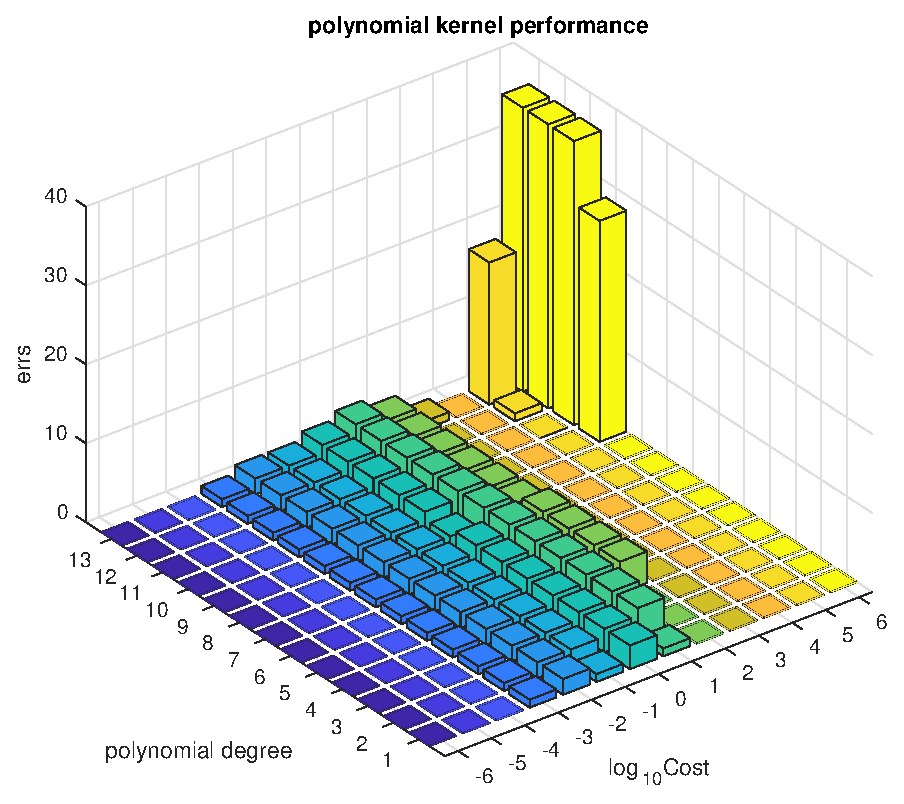
\includegraphics[width=.7\textwidth]{figure/polynomial_performance_s.eps}
\caption{polynomial performance signum}
\label{ps}
\end{figure}
\begin{figure}
\centering
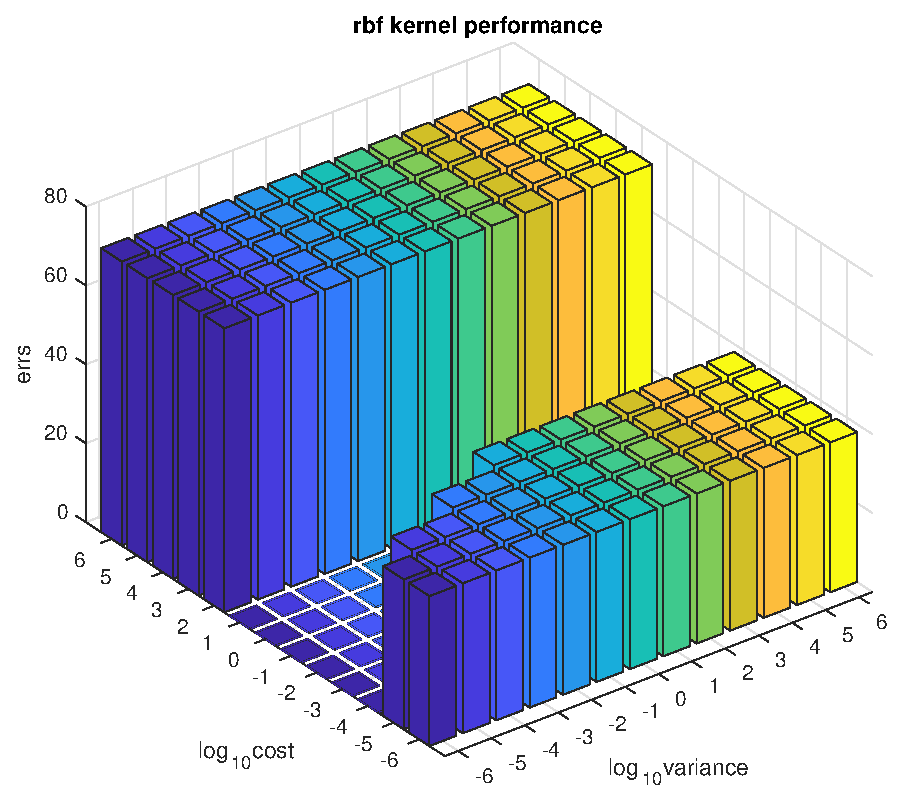
\includegraphics[width=.7\textwidth]{figure/rbf_performance_s.eps}
\caption{rbf performance signum}
\label{rs}
\end{figure}

Using the soft-margin, the performances are shown as in $\ref{l}$, $\ref{p}$, $\ref{r}$.
\begin{figure}
\centering
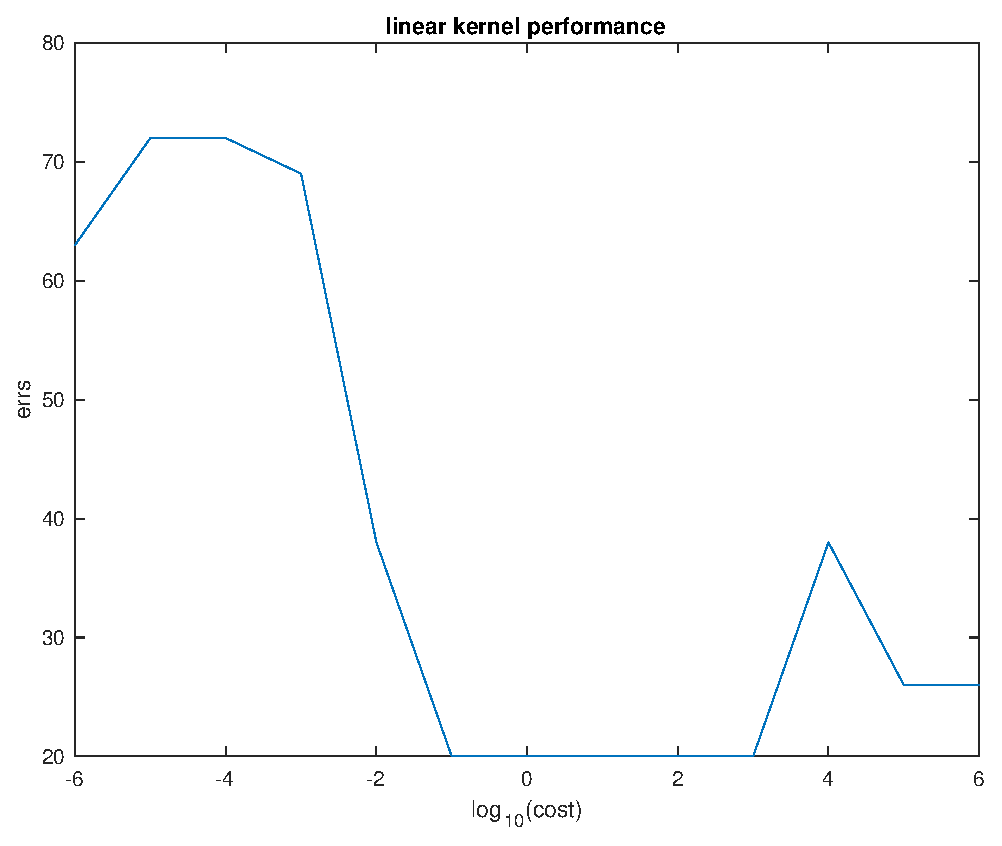
\includegraphics[width=.7\textwidth]{figure/linear_performance.eps}
\caption{linear performance softmargin}
\label{l}
\end{figure}
\begin{figure}
\centering
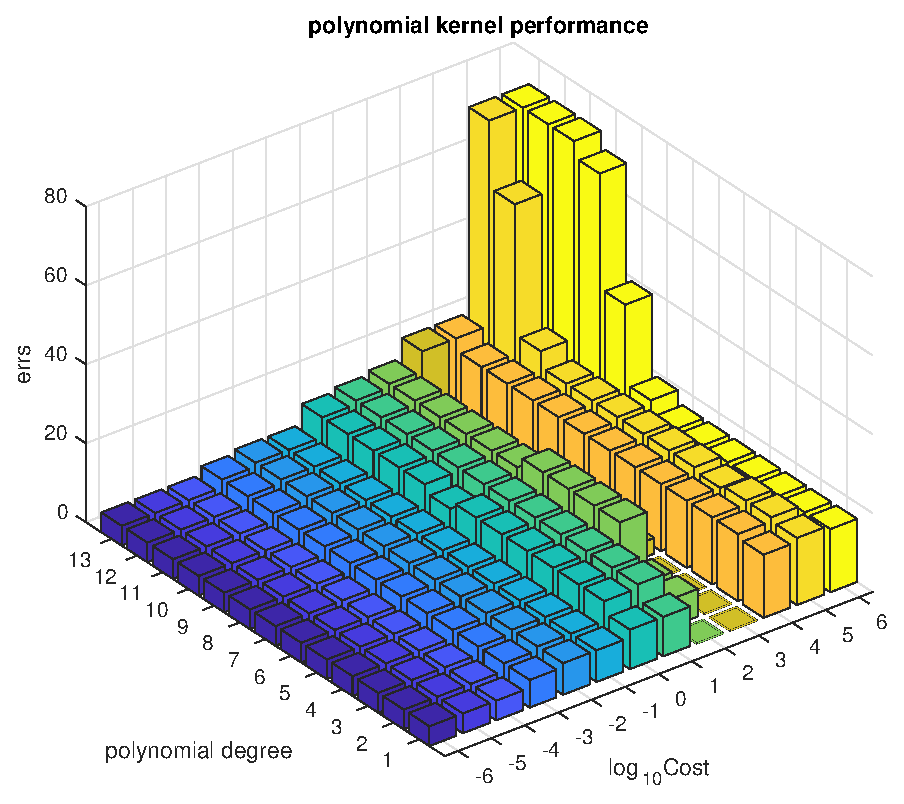
\includegraphics[width=.7\textwidth]{figure/polynomial_performance.eps}
\caption{polynomial performance softmargin}
\label{p}
\end{figure}
\begin{figure}
\centering
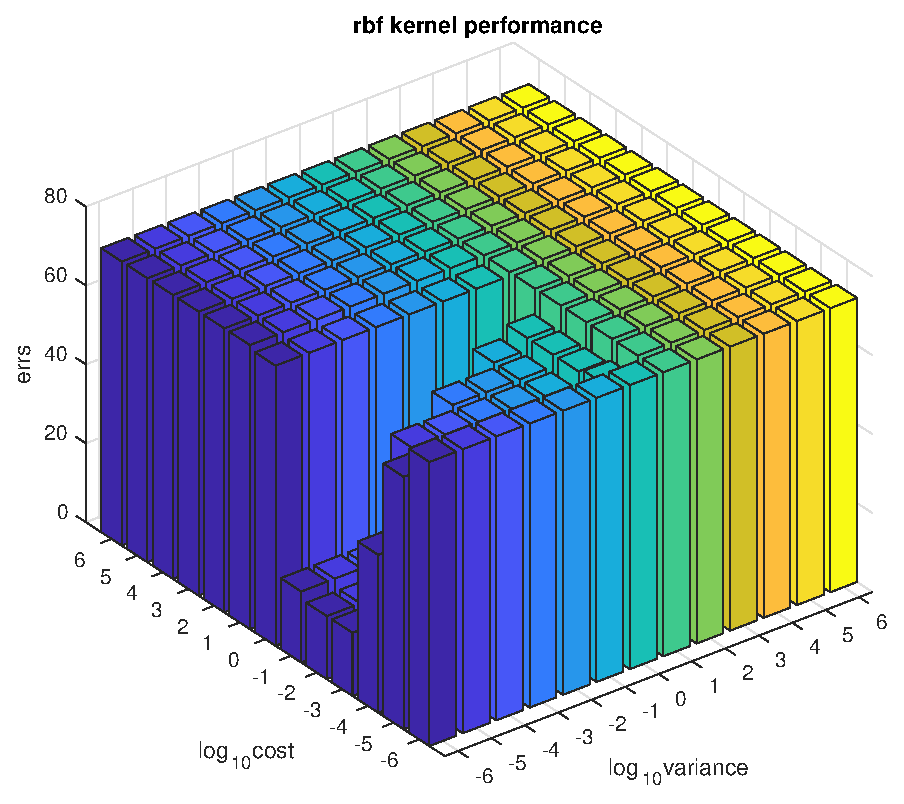
\includegraphics[width=.7\textwidth]{figure/rbf_performance.eps}
\caption{rbf performance softmargin}
\label{r}
\end{figure}

$\ref{ls}$ shows that when output $f(x)$ is as 

\begin{equation}
f(x) = sign(\sum_{t}\alpha_t y_t <x_t,x> ) \nonumber
\end{equation}

The SVMs perform well when $\log_{10}C \in (-2, 4)$ as the error becomes 0 within that interval.

Nevertheless there's some slight difference in $\ref{l}$ as the $f(x)$ becomes
\begin{equation}
f(x) = \left\{\begin{aligned}{ &+1 \quad &\sum_{t} \alpha_t y_t <x_t,x>-1>0 \\ &-1 \quad &\sum_{t} \alpha_t y_t <x_t,x>+1<0  \\ &\sum_{t} \alpha_t y_t <x_t,x> \qquad&else}\end{aligned} \nonumber
\end{equation}

In $\ref{p}$ 
\begin{equation}
 f(x) = \left\{\begin{aligned}{ &+1 \quad &\sum_{t} \alpha_t y_t (<x_t,x>+1)^n+b_0-1>0 \\ &-1 \quad &\sum_{t} \alpha_t y_t (<x_t,x>+1)^n+b_0+1<0  \\ &\sum_{t} \alpha_t y_t (<x_t,x>+1)^n+b_0 \quad&else}\end{aligned} \nonumber
\end{equation}

In $\ref{r}$ 
\begin{equation}
 f(x) = \left\{\begin{aligned}{ &+1 \ &\sum_{t} \alpha_t y_t \exp(\frac{-\lVert x_t-x\rVert^2}{2\sigma^2})+b_0-1>0 \\ &-1 \ &\sum_{t} \alpha_t y_t \exp(\frac{-\lVert x_t-x\rVert^2}{2\sigma^2})+b_0+1<0  \\ &\sum_{t} \alpha_t y_t \exp(\frac{-\lVert x_t-x\rVert^2}{2\sigma^2})+b_0 \quad&else}\end{aligned} \nonumber
\end{equation}

Since the classifier is more strict, there are generally greater recognition errors in $\ref{p}$ and $\ref{r}$. It can be denoted in both $\ref{p}$ and $\ref{ps}$ that the setting where $ p \leq 5 \ and \ 10^2 \leq C \leq10^4$ gives the best polynomial performance. When it comes to rbf kernel, the $C$ should be ranging from $10^{-4}$ to $10^{1}$ while $\sigma$ seems to have less effect on the performance according to $\ref{rs}$.

Conclusion:
\begin{enumerate}
\item linear \qquad $C \in (10^{-2}, 10^4)$.

\item polynomial \qquad $p \leq 5 \ and \ 10^2 \leq C \leq10^4$.

\item rbf \qquad $C \in (10^{-4} , 10^1) \ and \ \sigma < 10^{-3}$.
\end{enumerate}

\section{Problem 3: PCA}

 Reconstruct the data using PCA with least squares error using only the mean and a linear combination of the top 3 eigenvectors. Show 10 different images before and after reconstruction.
 
\begin{figure}[h]
\centering
\subfigure[1]{
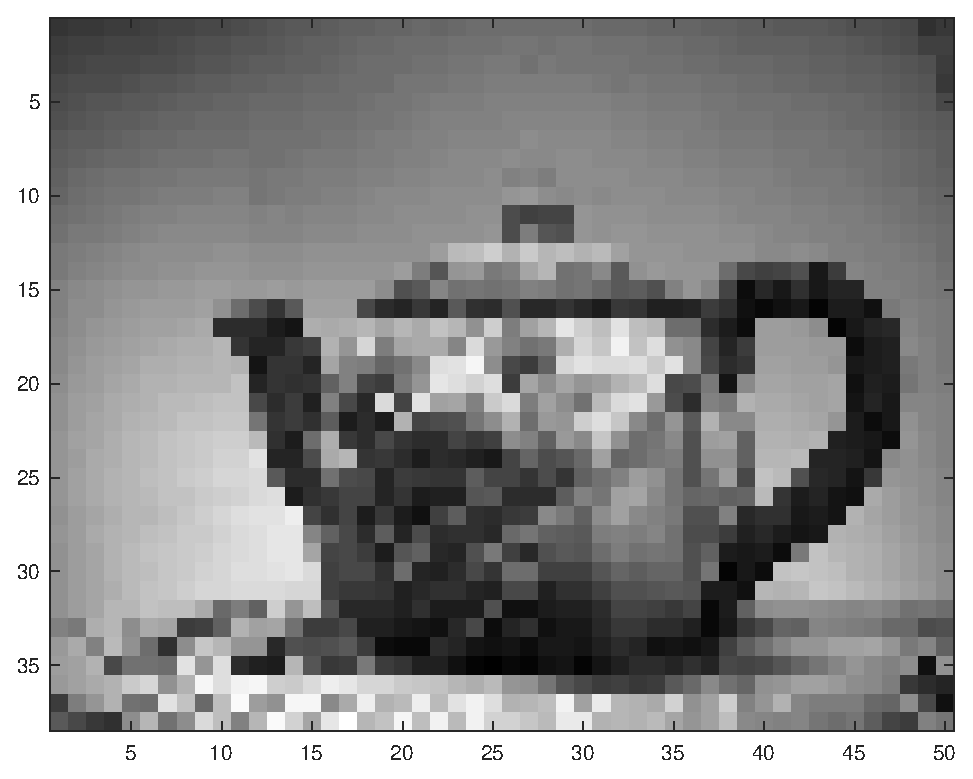
\includegraphics[width = .45\textwidth]{figure/1.eps}
}
\subfigure[1 reconstructed]{
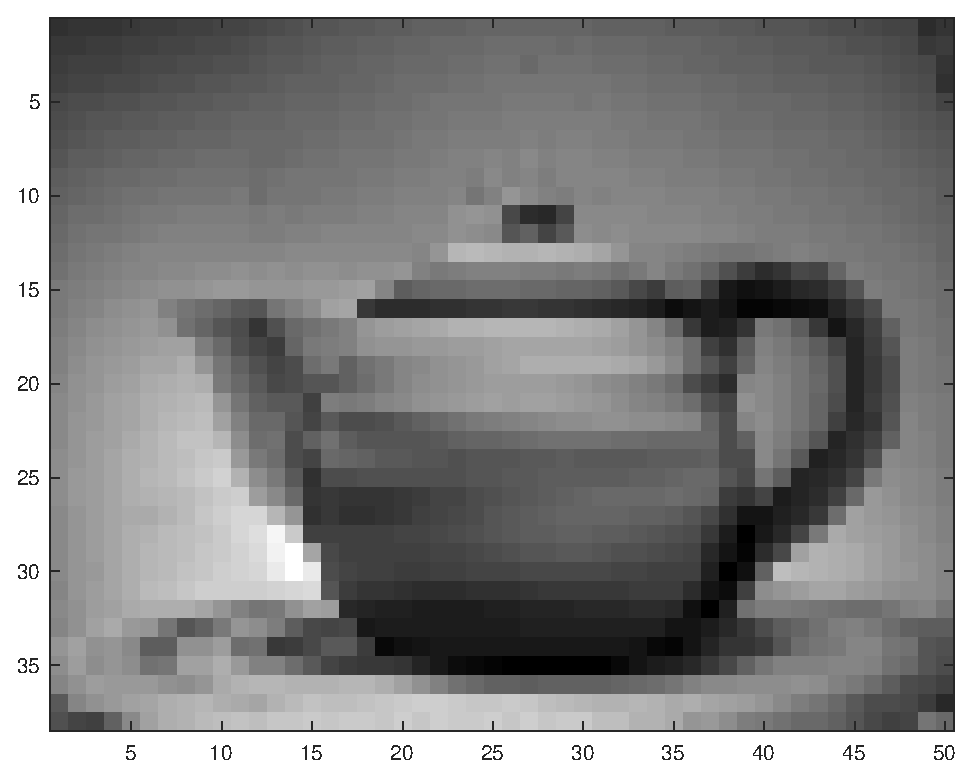
\includegraphics[width = .45\textwidth]{figure/1_rec.eps}
}
\\
\centering
\subfigure[2]{
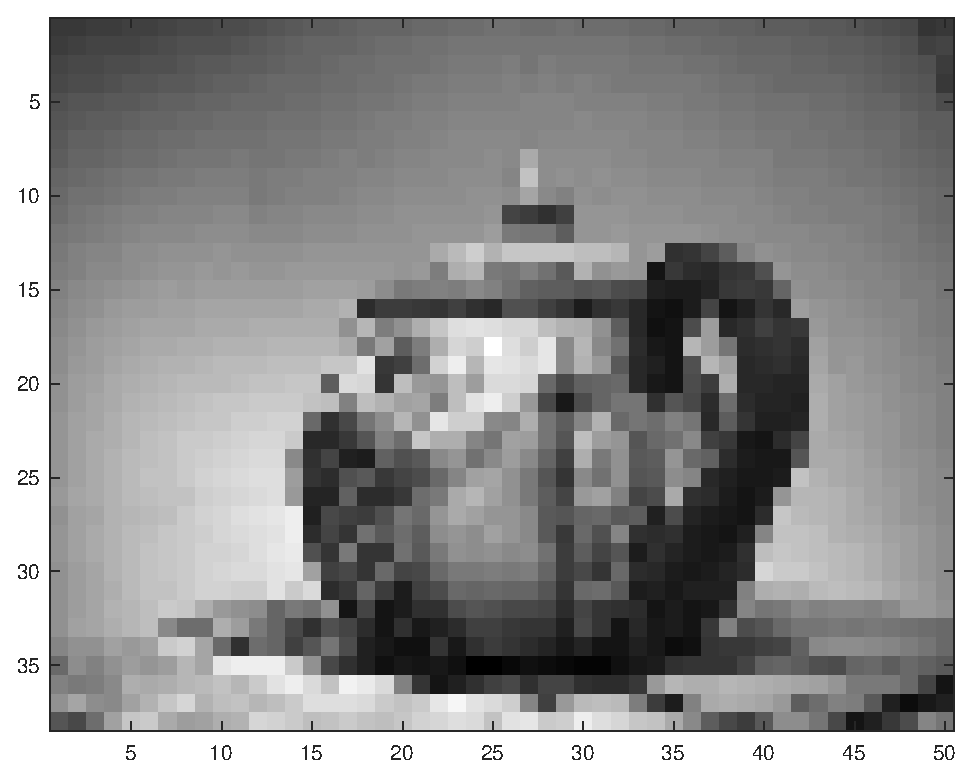
\includegraphics[width = .45\textwidth]{figure/2.eps}
}
\subfigure[2 reconstructed]{
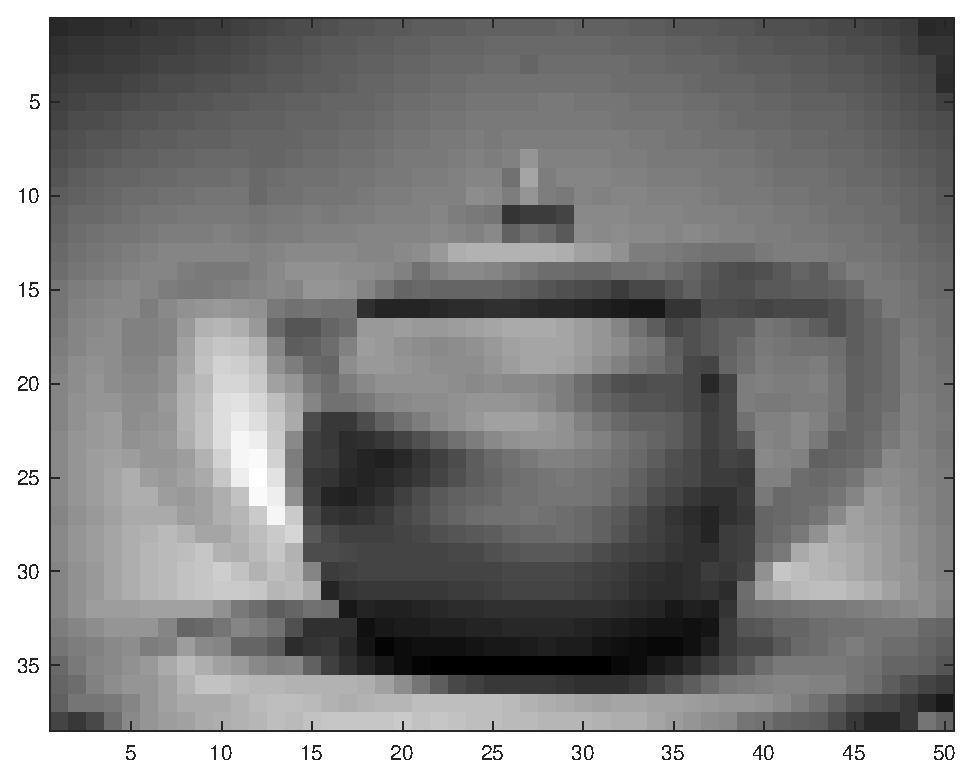
\includegraphics[width = .45\textwidth]{figure/2_rec.eps}
}
\end{figure}
\\
\begin{figure}[h]
\centering
\subfigure[3]{
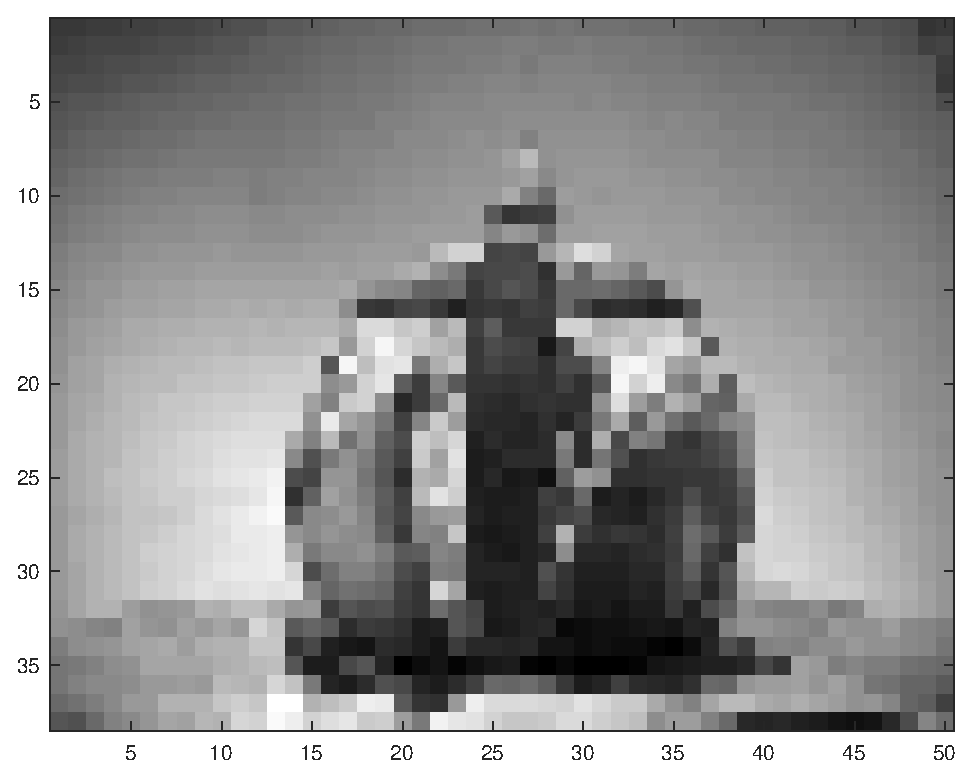
\includegraphics[width = .45\textwidth]{figure/3.eps}
}
\subfigure[3 reconstructed]{
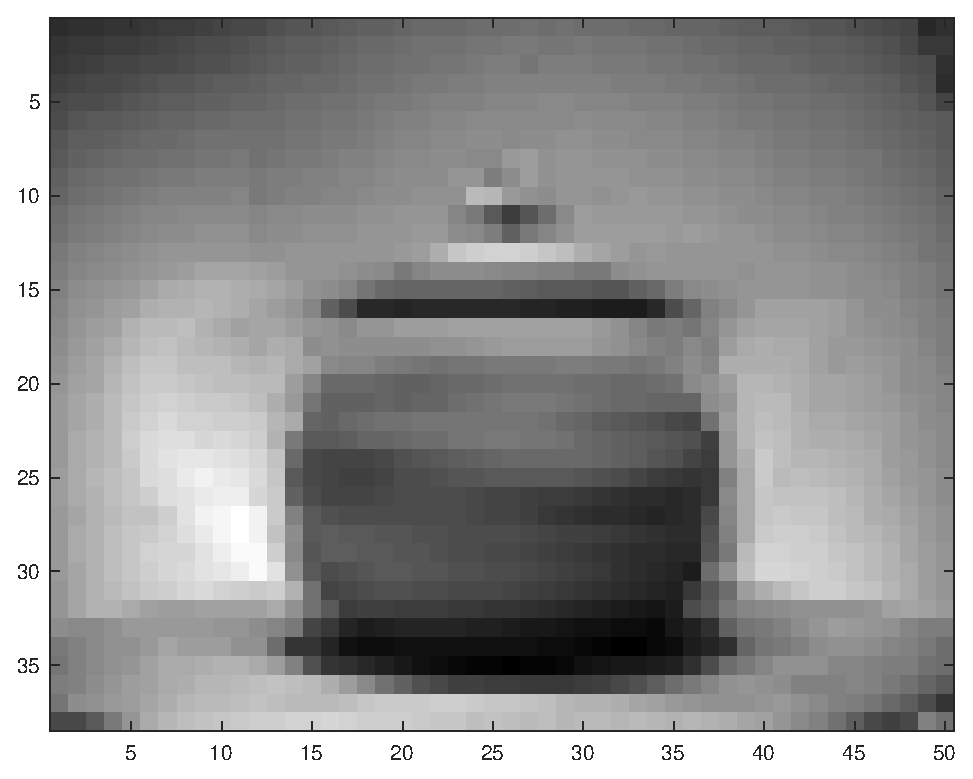
\includegraphics[width = .45\textwidth]{figure/3_rec.eps}
}
\end{figure}
\\
\begin{figure}[h]
\centering
\subfigure[4]{
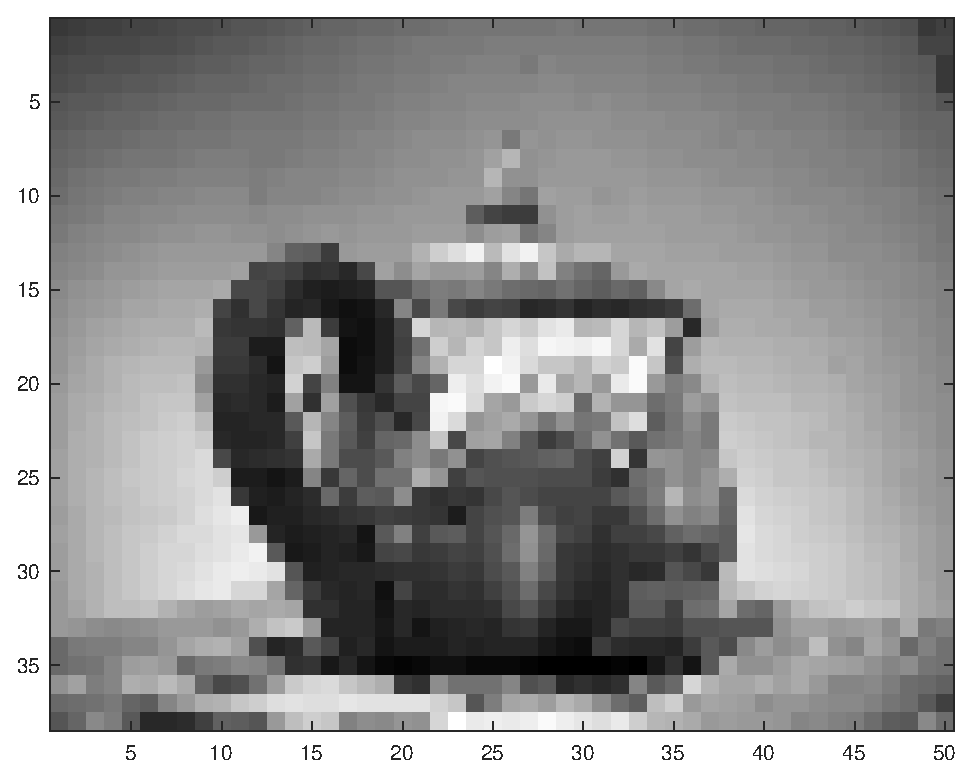
\includegraphics[width = .45\textwidth]{figure/4.eps}
}
\subfigure[4 reconstructed]{
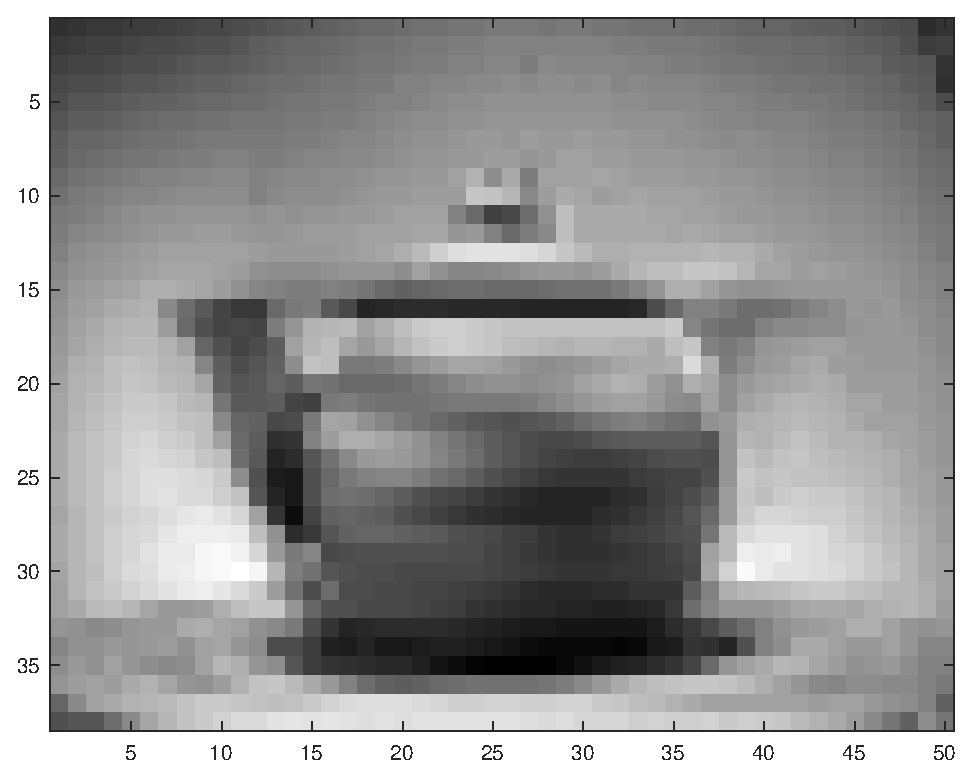
\includegraphics[width = .45\textwidth]{figure/4_rec.eps}
}
\end{figure}

\begin{figure}[h]
\centering
\subfigure[5]{
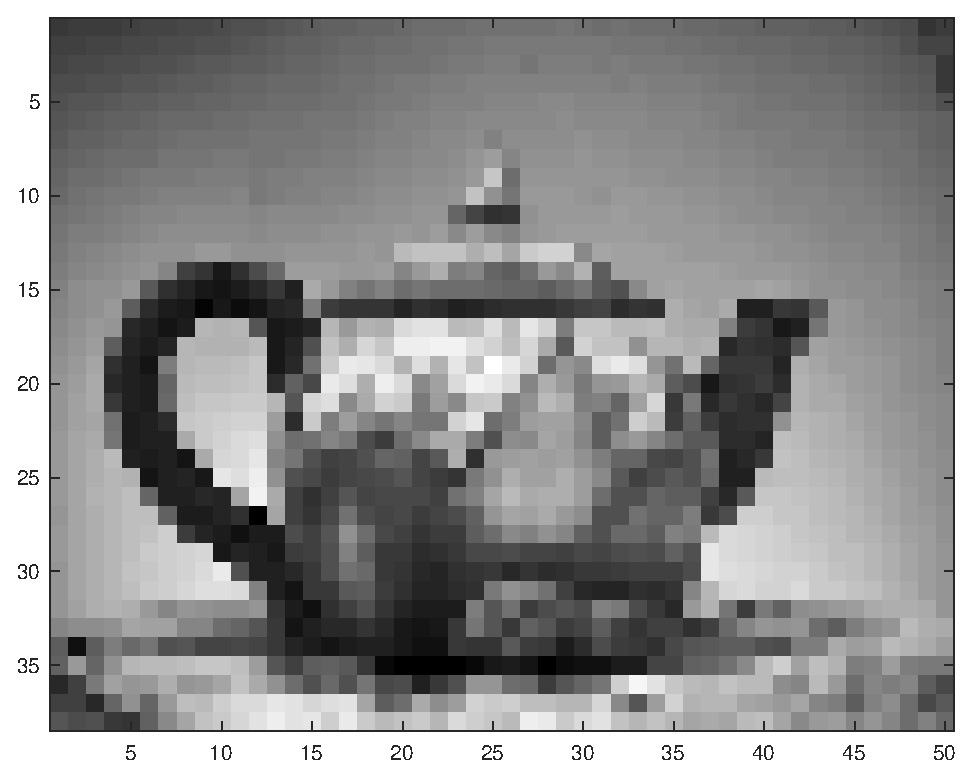
\includegraphics[width = .45\textwidth]{figure/5.eps}
}
\subfigure[5 reconstructed]{
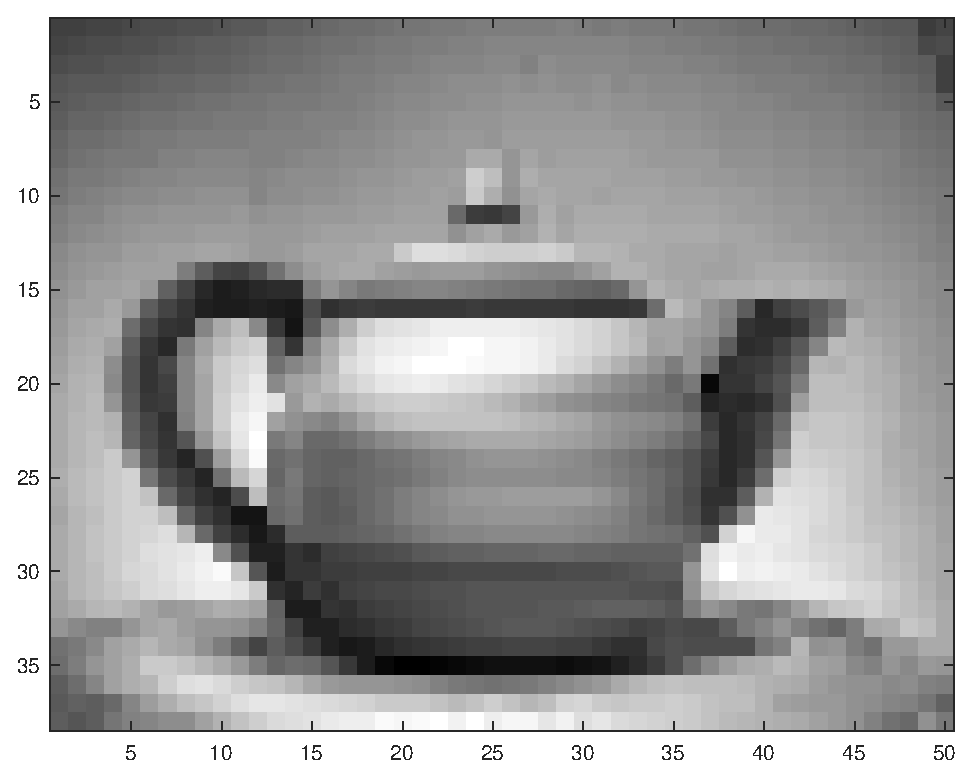
\includegraphics[width = .45\textwidth]{figure/5_rec.eps}
}
\end{figure}
\\
\begin{figure}
\centering
\subfigure[6]{
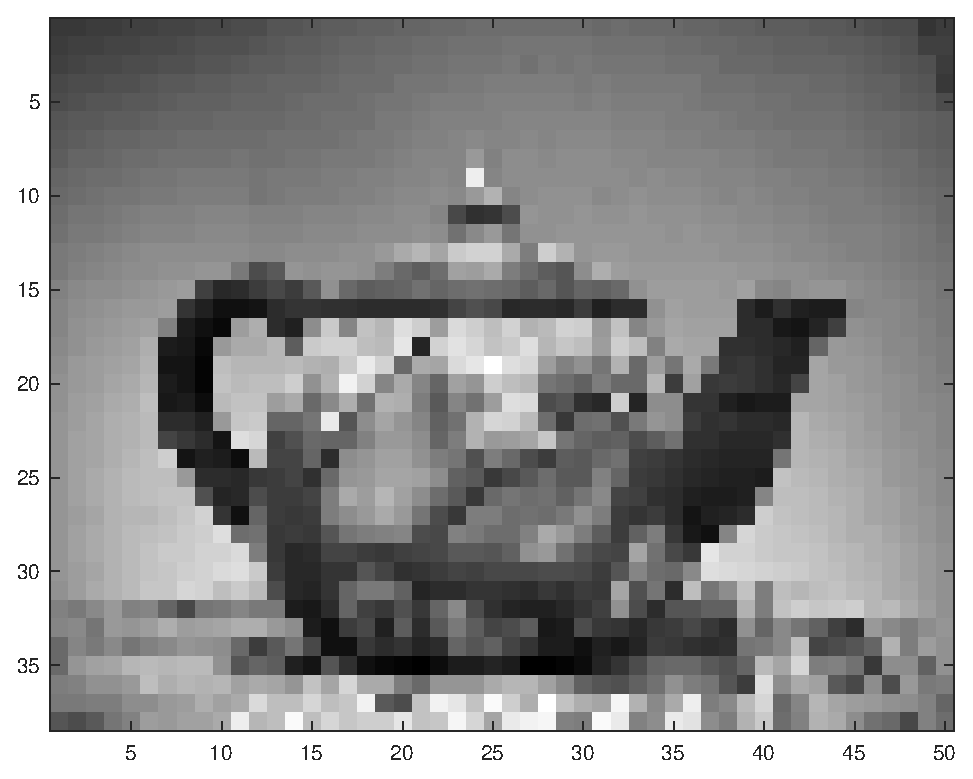
\includegraphics[width = .45\textwidth]{figure/6.eps}
}
\subfigure[6 reconstructed]{
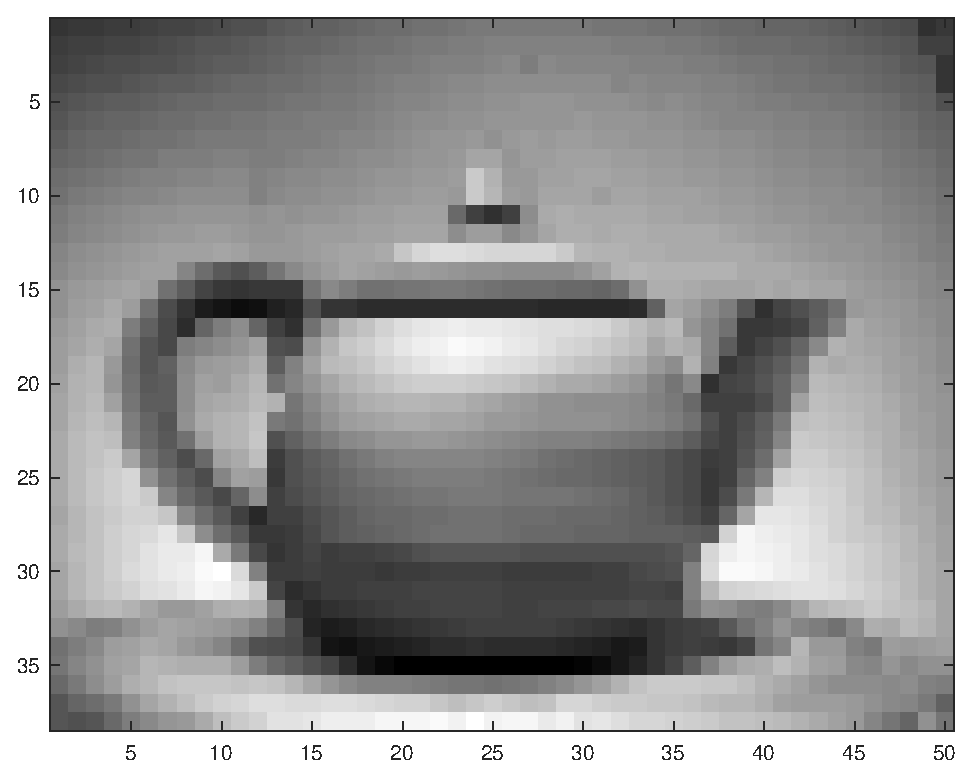
\includegraphics[width = .45\textwidth]{figure/6_rec.eps}
}
\end{figure}
\\
\begin{figure}[h]
\centering
\subfigure[7]{
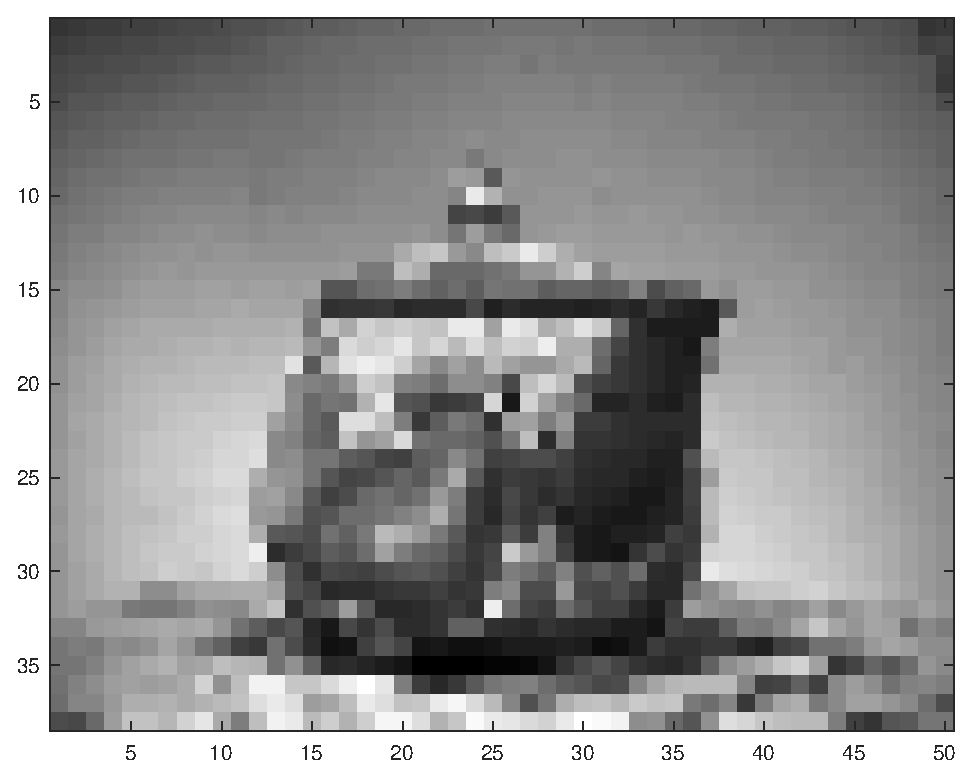
\includegraphics[width = .45\textwidth]{figure/7.eps}
}
\subfigure[7 reconstructed]{
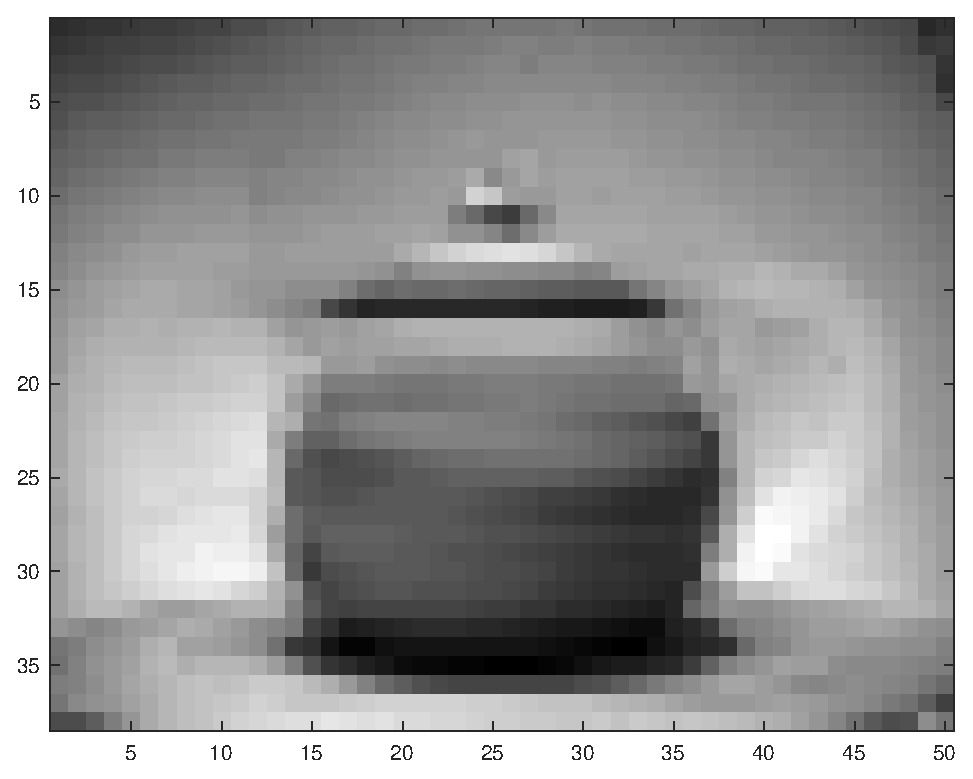
\includegraphics[width = .45\textwidth]{figure/7_rec.eps}
}
\end{figure}
\\
\begin{figure}[h]
\centering
\subfigure[8]{
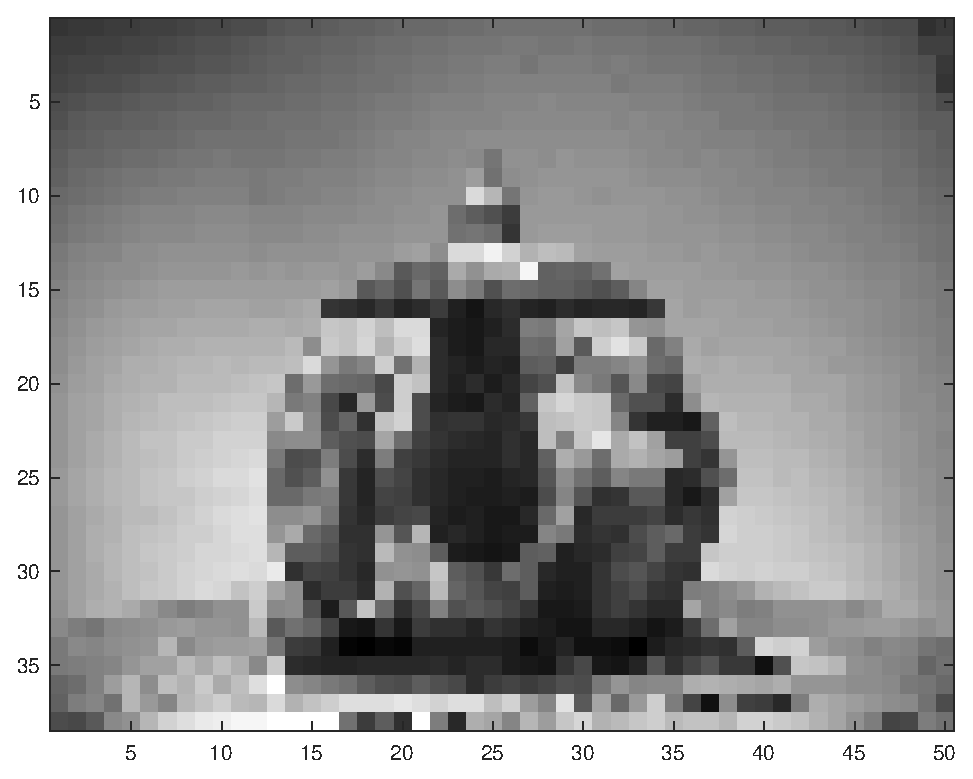
\includegraphics[width = .45\textwidth]{figure/8.eps}
}
\subfigure[8 reconstructed]{
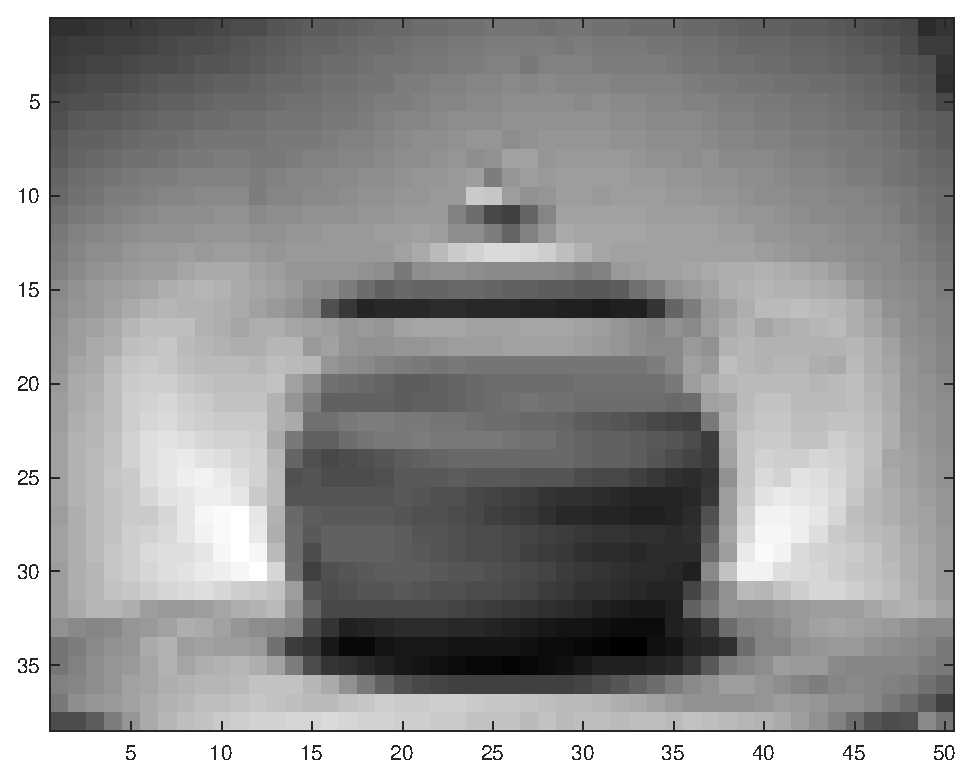
\includegraphics[width = .45\textwidth]{figure/8_rec.eps}
}
\end{figure}
\begin{figure}[h]
\centering
\subfigure[9]{
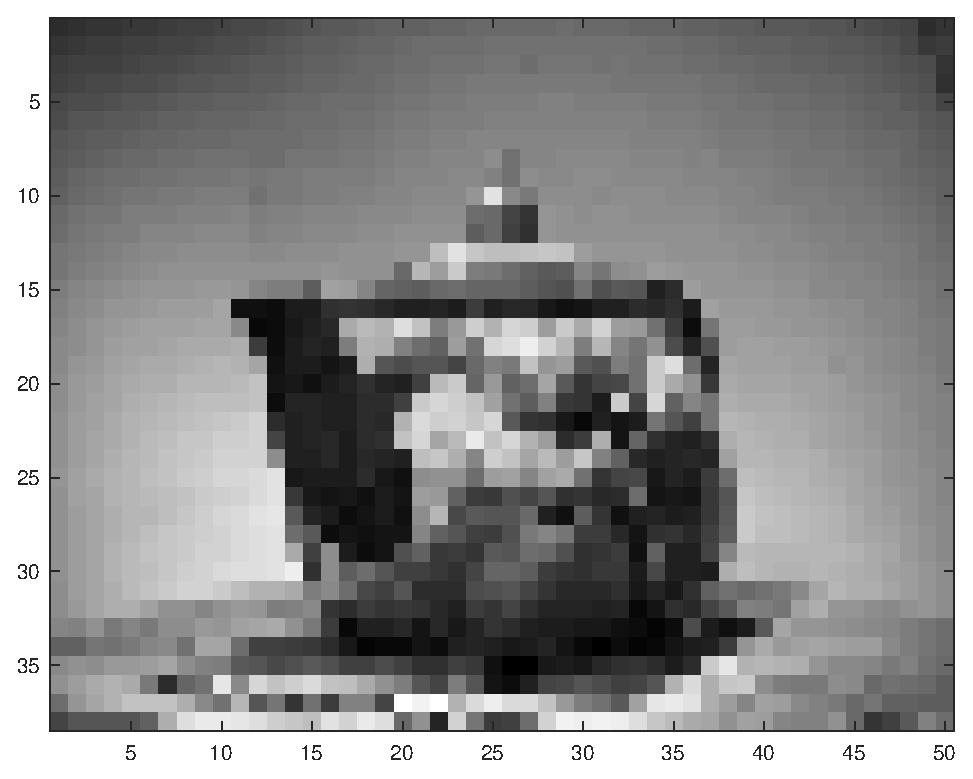
\includegraphics[width = .45\textwidth]{figure/9.eps}
}
\subfigure[9 reconstructed]{
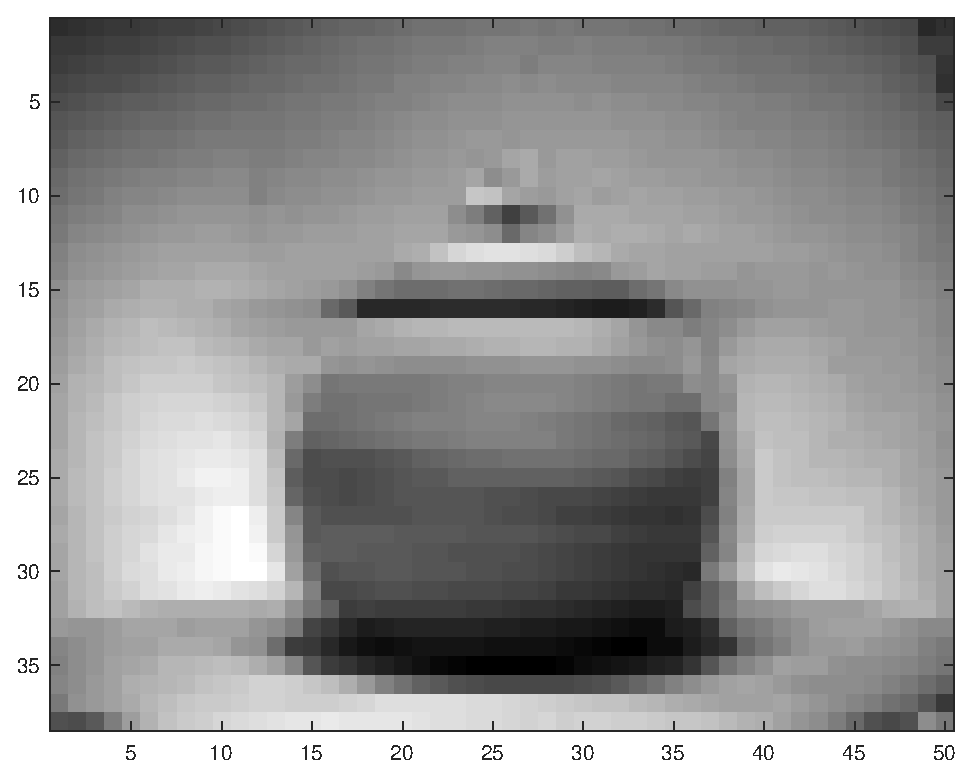
\includegraphics[width = .45\textwidth]{figure/9_rec.eps}
}
\end{figure}
\\
\begin{figure}[h]
\centering
\subfigure[10]{
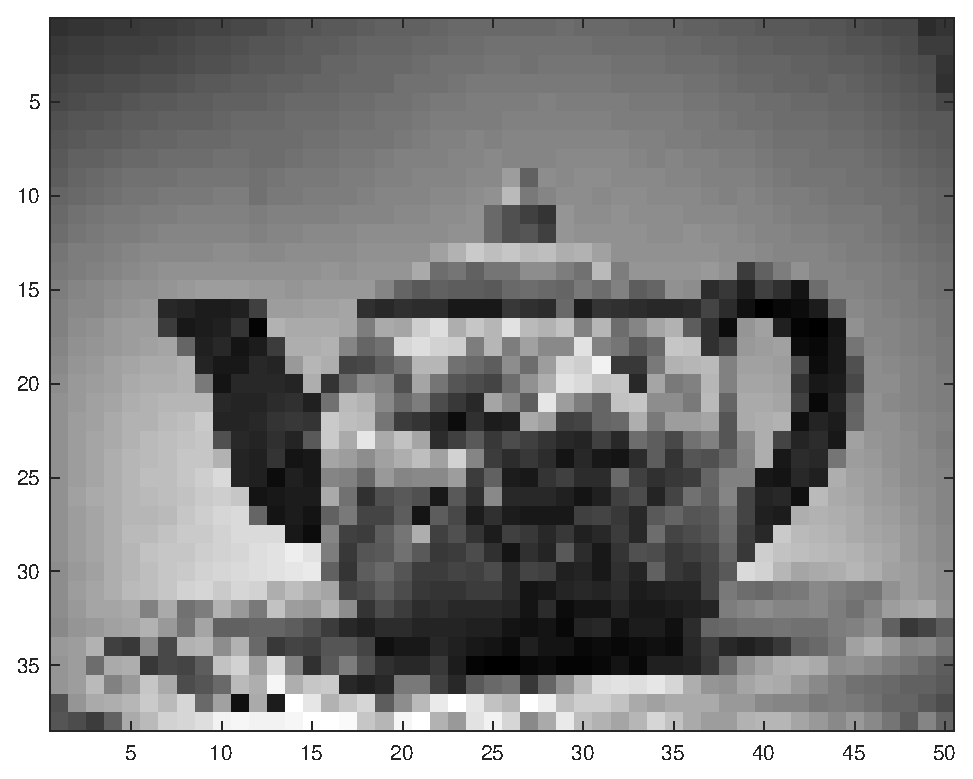
\includegraphics[width = .45\textwidth]{figure/10.eps}
}
\subfigure[10 reconstructed]{
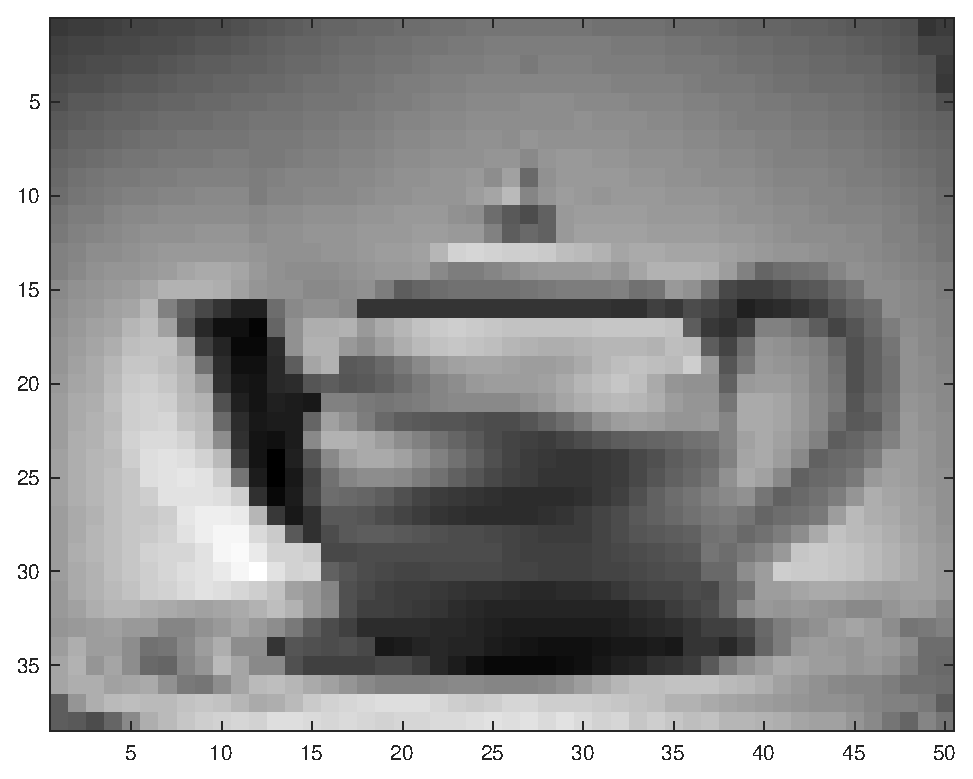
\includegraphics[width = .45\textwidth]{figure/10_rec.eps}
}
\end{figure}

Discussion: PCA reserves the main information of the data, which contains the mean value and featured terms, the mean value can be intuitively viewed as a spinning teapot which has no spout and handle, and the featured terms can be viewed as the information (pixels and positions) of its handle and spout. By constructing covariance matrix we obtain the self-derivate and the co-derivate on every dimension of the datasets, and for every data point we pick the most effective 3 directions by Eigen-decomposition of the covariance matrix to reconstruct it.

\end{document}